\documentclass[thesis.tex]{subfiles}
\begin{document}

\chapter{Methodology}\label{chap:basics}

In this chapter we describe in detail how each step of our proposed pipeline is realized. In the first step of the pipeline we obtain cross-sections by going along the centerlines in the volume data. Then, we extract the contours of the TL and FL from the obtained cross-sections. In the third step of the pipeline we represent the extracted contours using chain codes. We then apply a fourier transform on the chain codes to obtain EFDs. In the fifth step we then use the EFDs to approximate the lumen shapes and correct the overlapping contours that might occur. The result is then be used for visualization, rendering, and interpolation. We also add a vessel wall around the recontructed and corrected contours. An overview of this pipeline is shown in figure \ref{fig:pipeline}. We demonstrate all methods on a phantom data set thoughout this chapter. 

\begin{center}
\begin{tikzpicture}[node distance = 3cm, auto] \label{fig:pipeline}

    % Place nodes
    \node [block] (init) {Obtain cross-sections};
    \node [cloud, left of=init] (expert) {expert};
    \node [block, below of=init] (contours) {Extract contours};
    \node [block, below of=contours] (chaincode) {Convert contours to chain codes};
    \node [block, below of=chaincode] (efds) {Compute EFDs};
    \node [decision, below of=efds, node distance=4cm] (decide) {Cross-sections obtained with TCL ?};
    \node [block, below of=decide, node distance=4cm] (overlap) {Correct overlapping contours};
	\node [block, below of=overlap] (vesselwall) {Create vessel wall};
	\node [block, below of=vesselwall] (use) {Use EFDs for rendering etc.};
    % Draw edges
    \path [line] (init) -- (contours);
    \path [line] (contours) -- (chaincode);
    \path [line] (chaincode) -- (efds);
	\path [line] (efds) -- (decide);
	\path [line] (overlap) -- (vesselwall);
	\path [line] (vesselwall) -- (use);
    %\path [line] (decide) -- node {no} (use);
    \path [line] (decide) -- node {yes}(overlap);
    %\path [line,dashed] (expert) -- (init);
\end{tikzpicture}
\end{center}


\section{Obtaining Cross-Sections}
In this step of the pipeline we describe how cross-sections are obtained from the provided volume data. Each dataset of the provided data contains three centerlines, the centerline of the FL, the centerline of the TL , and the TCL. The TCL interpolates points that lie between the centerlines of the TL and FL. All centerlines are modeled by interpolating B-Splines. To obtain cross-sections, we go along a centerline using a fixed step size and compute a local coordinate frame at each position that we visit on the centerline. The step size is computed by dividing the length of the centerline by the number of desired cross-sections, which is a parameter the user can specify. This ensures that each lumen is represented by the same amount of cross-sections. Each local coordinate frame consist of two 3-dimensional vectors, which are orthogonal to the centerline at the centerline position they were obtained. The two vectors define the x- and y-axis of the cross-section in the 3-dimensional space of the volume data. Starting from the centerline position we sample the volume in the directions of the positive and negative x- and y-axes of the cross-section. By doing this we obtain the positions of the cross-section pixels in the 3-dimensional space of the volume data. The positive and negative x- and y-axes are used because we want the centerline to be in the center of the cross-section. The obtained 3-dimensional positions have floating point precision and are truncated to their integer, which corresponds to the the position of a voxel in the volume. The final intensity of a pixel in the cross-section is then obtained by trilinear interpolation of the non-zero values of this voxel and the 7 neighboring voxels that form a volume cell. An example of the obtained cross-sections is shown in figure \ref{fig:obliqueslices}\\

\begin{figure}[h]
\centering
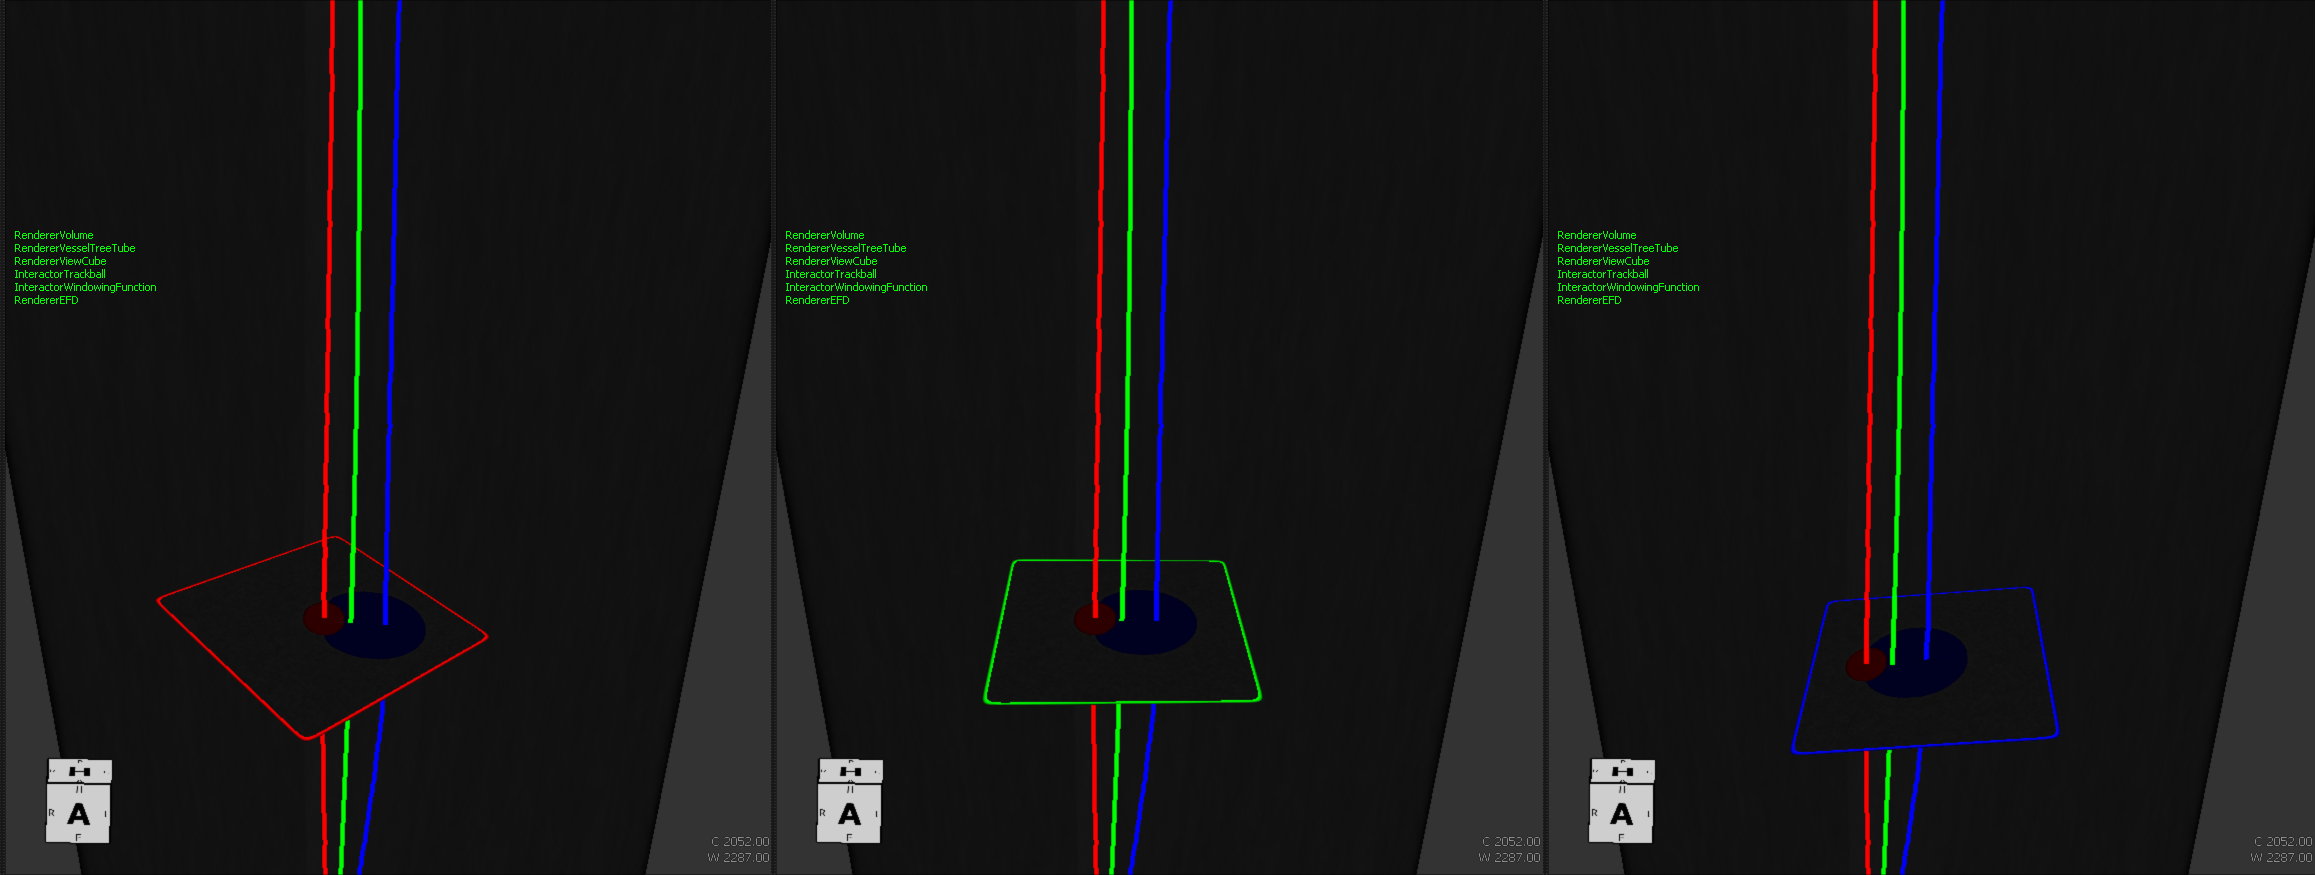
\includegraphics[width=\textwidth]{obliqueslices.PNG}
\caption{The three centerlines of our phantom dataset. The TL centerline, TCL, and FL centerline are colored red, green, and blue respectively. A cross-section is shown for each centerline. The cross-sections are orthogonal to their corresponding centerline, but not necessarily to other centerlines. That is why the cross-section of the TL and TCL look different, even though the same offset was used. The cross-section of the FL uses a different offset, because the FL centerline is shorter than the other centerlines in the dataset.}
\label{fig:obliqueslices}
\end{figure} 

By default we use the TCL to obtain cross-sections, but the user can also choose to use the centerlines of the TL and FL instead. We chose the TCL as default, because the obtained cross-sections are easier to use in the other steps of the pipeline.
In the following we describe problems that can occur when obtaining cross-sections and how we solved or avoided them. 

\subsection{Problems when obtaining cross-sections}

\textbf{Overlapping Cross-sections} 

Overlapping cross-sections can occur at positions the centerline has high curvature. They can be problematic, because some surface rendering algorithmns for example marching cubes work by connecting points from consecutive cross-sections. However, when cross-sections overlap, inner structures within the surface occur. These inner structures make the surface useless for severeal appplications. When simulating the flow of blood within the lumen for example, the result is influenced by the inner structures. Therefore, only surfaces without inner structures are desired. A possible solution was proposed by the authors of \cite{wu2010curvature}. They propose to use an adaptive step size that depends on the gaussian curvature of the centerline to bi-directionally down-sample the centerline, before obtaining cross-sections. This ensures that cross-sections are far apart in regions of high curvature. \\
We avoided this problem by not storing the correspondence of contour pixels to their cross-section. This means the extracted contours are interpreted as a point cloud. We assume that a point cloud is sufficient to create a smooth surface without inner structures.  

\textbf{Distortion of lumen} 

Lumen can appear distorted within the cross-sections. Each cross-section is oriented orthogonal to the centerline that was used to obtain them. However, they are not oriented orthogonal to other centerlines. If a cross-section is not oriented orthogonal to the centerline of a lumen, the lumen appears elongated in the cross-section, because the diameter of the lumen in direction of the cross-section is larger than in the direction orthogonal to the centerline of the lumen. This is illustrated in figure \ref{fig:cross-section_distortion}. This means that when we use the TCL to obtain cross-sections, the cross-sections are not oriented orthogonal to the centerlines of the FL and TL and both lumen may appear elongated. If we use the TL centerline, the cross-sections are not orthogonal to the FL centerline and the FL may appear elongated. If we use the FL centerline, the cross-sections are not orthogonal to the TL and the TL may appear elongated. Elongated contours are problematic because they make estimation of the lumen size difficult. Also, an elongated lumen can mean that the used step size is too large to appropriately sample the elongated lumen, resulting in a loss of features of the elongated lumen. \\ Currently we do not solve or avoid this problem. We do not estimate the size of the lumen. We assume that the lumen surface can be more accurately reconstructed by using the centerline of the lumen that is to be reconstructed than when using any other centerline. We also assume that the TCL is the second best choice for reconstruction: Since the TCL interpolates points that lie between the other centerlines, the angle between cross-sections obtained from the FL centerline and cross-sections obtained from the TL centerline should also be interpolated by cross-sections obtained from the TCL. This is illustrated in figure .... .
\todo[inline]{todo: Keine ahnung ob man das so versteht. Bild einfügen}

\textbf{Choosing of the Centerline}

As we explained in the previous sections no matter which centerline we choose to obtain cross-sections at least one lumen will appear elongated in the cross-sections. For surface reconstruction we can use the centerlines of the respective lumen that is to be reconstructed for best results, but the obtained cross-sections cannot be used in all steps of the pipeline. 
When we use the TCL to obtain cross-section we only have one step size that is used while going along the spline. When we use the centerlines of the FL and TL instead, we have two different step sizes, because the step size depends on the length of the respective centerline. These differences make it complicated to use the cross-sections obtained from the centerlines of the FL and TL in some steps of the pipeline. For example in the step of the pipeline in which we correct the overlapping of the reconstructed contours we have to identify both lumen in each cross-section. In the case the cross-sections were obtained by using centerlines of the FL and TL, we can either ignore the parameter that controls the number of cross-sections to be used and process all cross-sections, or we have to decide which cross-sections to use.
The centerline of the TL is usually longer than the centerline of the FL. This means we cannot assume that the n-th cross-section of the TL is anywhere near the n-th cross-section of the FL. If we were to use only cross-sections from the FL centerline, we would not cover the whole TL. On the other hand, if we were to use only cross-sections of the TL centerline, the step size could be too large and some important features of the FL could be skipped. By using the TCL as default we avoid those problems. In case the user wants to use the respecitve lumen centerlines instead of the TCL those steps are currently skipped. An example of a cross-section can be seen in figure \ref{fig:cross-section}.

\begin{figure}[h]
\centering
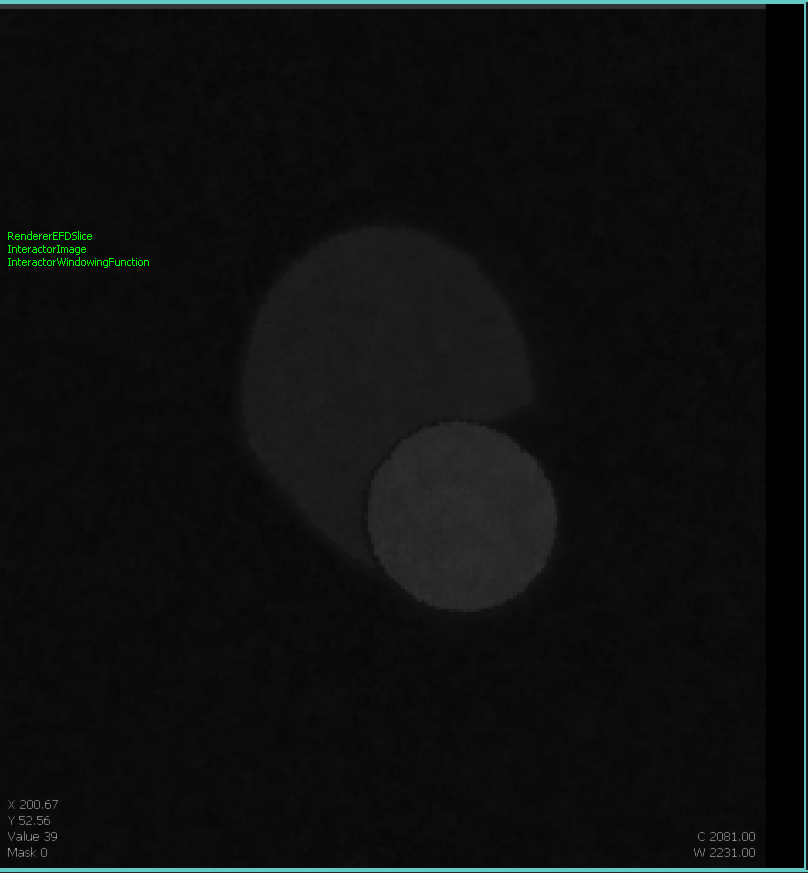
\includegraphics[width=\textwidth/2]{cross-section249.png}
\caption{A cross-section of the phantom data set. In the center both lumen are visible. The TL is the almost perfect circular lumen with brighter intensity values than the FL. The FL is the non-circular lumen that winds arounds the TL.}
\label{fig:cross-section}
\end{figure}  

\begin{figure}[h]
\centering
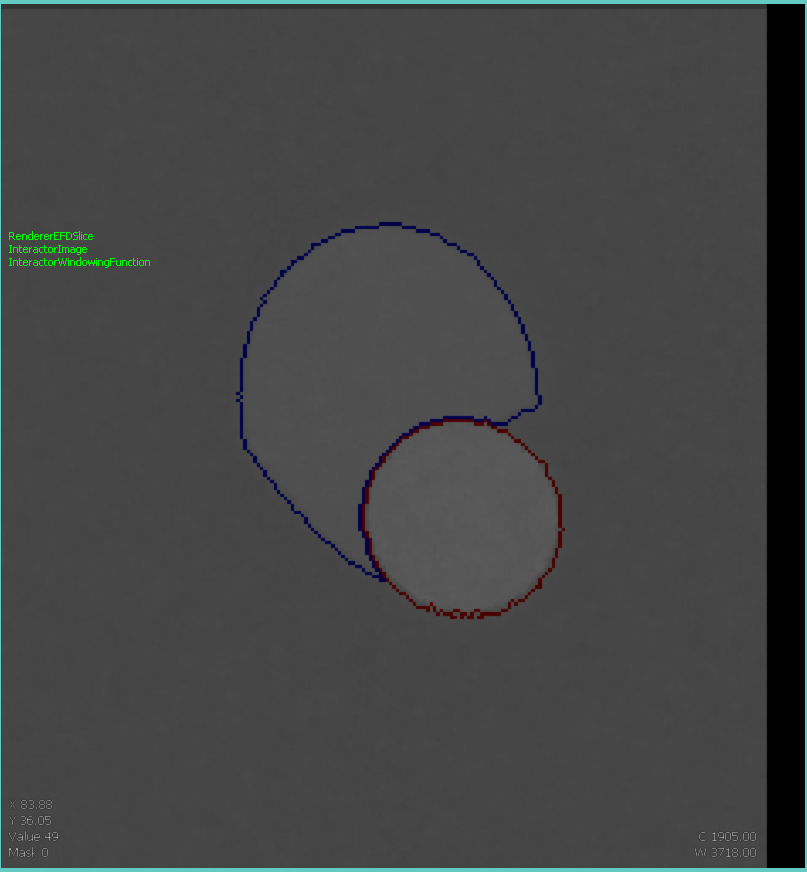
\includegraphics[width=\textwidth/2]{cross-section249_with_extracted_contours.png}
\caption{The same cross-section as in \ref{fig:cross-section} after extracting the lumen contours. In the center both lumen are visible and their respective contours overlayed. The contour of the FL is colored blue, while the contour of the TL is colored red. Compared to \ref{fig:cross-section} the windowing function was adjusted for better visibility of the contours.}
\label{fig:extracted_contours}
\end{figure} 

\section{Extracting Lumen Contours}
Cross-sections might migth intersect the same lumen at positions with high curvature as shown in figure \ref{}. This results in the appearence of the same lumen at several positions in the cross-sections. Therefore, before extracting the contour we first have determine the largest connected area of each lumen in the cross-section. We do this by iterating over the pixels until we find a pixel that belongs to a lumen. Since the data is segmentated, we can trivially identify such pixels. \\   

We use the contour tracing algorithm that we described in \ref{contourtracingalgorithm} to extract the lumen contours from the cross-sections. To select a starting pixel we iterate over the pixels from left to right, top to down until we find a contour pixel. By doing it this way we satisfiy the condition of the contour tracing algorithmn that the rear-left pixel relative to the starting pixel is not an inner-outer-corner pixel.
\todo[inline]{TODO: conditions in relative work} 
The result of applying the contour tracing algorithm is an ordered list of contour pixel positions and their classifications.
An example of the extracted contours can be seen in figure \ref{fig:extracted_contours}.

\section{Converting Contour to Chain Code}
After we extracted the contours of the cross-sections we convert them to chain codes. This is mainly done to represent the contour as a one-dimensional signal, so that we can apply the fourier transform. The Encoding Scheme we use is the Freeman Chain Encoding Scheme that we describe in section \ref{freeman}. The chain codes are only stored temporarily, so we do not need to normalize them in any way.

\section{Computing Elliptic Fourier Descriptors}
In this step we have to compute the EFDs that will be used to represent the shapes of the lumen. As the EFDs are a set of fourier coefficients, we have to use the Discrete Fourier Transform on the chain codes we obtained in the last step of the pipeline. More specifically, we use the DFT defined in \cite{giardinia}. We described how the authors applied the fourier transform on the freeman chain code in section \ref{elliptic_fourier_descriptors}. 

In our implementation we use equations \ref{eq:dft_dc} and \ref{eq:dft_coefficients} to obtain the fourier coefficients. We also use the fourier approximations in euqations \ref{eq:dft} to reconstruct the contour in a gapless manner, if it is necessary to do so. However, for most steps of our pipeline and for many rendering applications it is sufficient to reconstruct the signal using less reconstruction points. The main advantages of using less reconstruction points is the reduced memory consumption and faster processing due to the lower number of points that need to be processed. For this purpose we also implemented another fourier approximation that is very similar to the ones defined in \ref{eq:dft}. The only differences are that we set $t$ to be the index of the current reconstruction point and $T$ to be the total number of reconstruction points that should be used. This changes cause the reconstructed points to be placed equidistantly on the reconstructed contour and allow the user to freely adjust the total number of reconstruction points.\\ 

\section{Correcting of overlapping contours}
In this step we ensure that the reconstructed contours do not overlap. This can happen if not sufficient harmonics were used during the computation of the EFDs. For this purpose we iterate over the cross-sections and retrieve the EFDs that describe the contours found in the cross-sections. In our implementation the EFDs are stored in a way that allows us to do so. Additionally, we can differentiate to which lumen each EFD belongs. By doing the iteration using the cross-sections we end up with two EFDs in each iteration. The first EFD describes the FL contour in the current cross-section, while the other describes the lumen contour of the TL. 
The algorithm to correct the overlapping contours can be summarized in the following five steps:

\begin{enumerate}
\item Create a layer for each lumen and draw the reconstructed contours into the corresponding layer
\item Fill the area outside of the reconstructed contour
\item For the FL, fill the area inside of the contour
\item Combine the layers in a specific way
\item Search for the corrected contours in the combined layer
\end{enumerate}

We will now describe each of these steps in detail. In the first step we create an empty image for each of the EFDs. We refer to them as \textit{layers}. Each layer has the same size as a cross-section and is initially filled with black pixels. Then we reconstruct the contours for both lumen using the EFDs. The contours are reconstructed in a gapless manner and they are drawn into their corresponding layers. When drawing the reconstructed contours, it is important to ensure that the drawn contours can still be differentiated, for example by choosing different drawing colors / pixel intensities. 

In the second step, we want to fill the area outside of the contours in both layers. The reason for doing this is that we actually want to fill the area inside the FL. By filling the area outside of the contours,  we can trivially determine pixels inside of the contour. At the time of implementation we did not know of another way to do this. A possible different solution that we did not implement would be to use the methode described in \cite{inside_contour}.  To fill the area outside the  contours we determine a pixel outside the contour, that is used as a starting pixel for the area filling. We determine this pixel by iterating over the pixels in each layer until we find a pixel belonging to the reconstructed contour. In our implementation we iterate over the pixels from left to right, top to down. Therefore, when we find a pixel we can ensure that the pixel above the found pixel is a black pixel that lies outside of the contour.The only exception is when the found pixel is on the top border of the layer, but that would mean that the cross-sections might be too small to fit the whole lumen. In that case the size of the cross-sections should be increased until the whole lumen fits inside without being on any border of the cross-section. \\  Starting from the black pixel above the found pixel we then fill the area outside of the contour with a specific color that differens from both colors that were used to draw the reconstructed contours. For the area filling we first add the black pixel to a list. Then we repeat the following: For each pixel on the list we check all pixels in the 4-neighborhood. If a checked pixel does not belong to the reconstructed contour and it's color is not the same as filling color, we add this pixel to the list and set the pixels color to be the filling color. After all pixels in the neighborhood of a pixel are checked, we remove the current pixel from the list. The algorithmn finishes when no more pixels are on the list. \\
After filling the area outside of the contour, we then want to fill the inside of the contour. Since the layers were initialized with black pixels, the inner area of both drawn reconstructed contours is filled with black pixels. That is why we only need to fill the area inside the contour for one of the layers. The color used for filling the inside of the contour is the same as the color that was used to draw the respective contour. We determine a pixel inside the contour by iterating over the pixels of the layer until we find a black pixel and we use this black pixel as a starting pixel to fill the inside area of the contour the same way we did when we filled the area outside of the contour. \\
In the next step we combine both layers. We first create an image with the same size as the layers and initialize it with black pixels. For each pixel of this empty image, we check the pixels in both layers that have the same coordinates as the current pixel in the new image. If the pixel in the TL layer belongs to the reconstructed TL contour or to the inside area of the reconstructed TL contour, we set the color of the current pixel to be the same as in the TL layer. Otherwise, we check if the pixel in the FL layer belongs to the reconstructed FL contour or the area inside of the FL contour. If it does, we set the color of the current pixel to be the same as in the FL layer. If none of these cases applies, we ignore the current pixel.\\
In the last step we extract the contours from the image that contains the combined layers. We do this by using the same method as in the second step of the pipeline. The obtained contours do not overlap, because the pixels in the TL layer were prioritized over the pixels in the FL layer when we combined both layers.        

\section{Generation of a vessel Wall}

\section{Rendering}

\section{Interpolation of Elliptic Fourier Coefficients}

\chapter{Results and Discussion}\label{chap:basics}

\chapter{Conclusion and Future Work:}\label{chap:basics}

\subfilebib % Makes bibliography available when compiling as subfile
\end{document}